\documentclass[11pt, a4paper]{article}
\usepackage{geometry}
\geometry{left=2cm, right=2cm, top=2cm, bottom=2cm}
\usepackage{amsmath}
\usepackage{graphicx}
\usepackage{array}
\usepackage[utf8]{inputenc}
\usepackage[T1]{fontenc}
\usepackage{hyperref}
\usepackage{tikz} % Useful for drawing flowcharts if needed, or just use space
\usetikzlibrary{shapes, arrows, positioning}
\usepackage{mhchem}

\title{Year 12 Chemistry - Worksheet 3 \\ Designing Syntheses: Flowchart Conventions}
\date{Module 7 - Lesson 3}
\author{Student Name: \underline{\hspace{5cm}} ID: \underline{\hspace{3cm}}}

\begin{document}
\maketitle

\section*{Part 1: Flowchart Conventions (Node: CHM\_M7\_SYNTH\_N1)}

Flowcharts are used to communicate multi-step synthesis pathways clearly and conventionally. Key conventions include:

\begin{itemize}
    \item \textbf{Compounds:} Represented inside boxes. Use either the correct IUPAC name or the structural formula. Be consistent.
    \item \textbf{Reactions:} Represented by arrows pointing from reactant(s) to product(s).
    \item \textbf{Reagents \& Conditions:} Written clearly above or below the reaction arrow corresponding to that specific step. Include necessary catalysts, solvents, heat ($\Delta$), UV light, etc.
    \item \textbf{Sequence:} Steps are arranged logically, usually top-to-bottom or left-to-right, showing the progression from starting material to final product via intermediates.
\end{itemize}

\textbf{Example Flowchart (Propane $\rightarrow$ Propanone):}

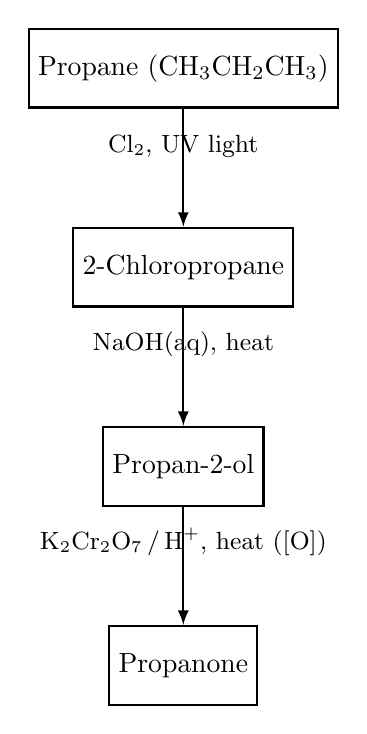
\begin{tikzpicture}[node distance=1.5cm, auto, >=latex,
    compound/.style={rectangle, draw, thick, minimum size=1cm, text centered},
    reagent/.style={above, midway, font=\small}]

    \node [compound] (propane) {Propane (\ce{CH3CH2CH3})};
    \node [compound, below=of propane] (chloro) {2-Chloropropane}; % Structure could be drawn instead
    \node [compound, below=of chloro] (propanol) {Propan-2-ol};
    \node [compound, below=of propanol] (propanone) {Propanone};

    \draw [->, thick] (propane) -- node [reagent] {\ce{Cl2}, UV light} (chloro);
    \draw [->, thick] (chloro) -- node [reagent] {NaOH(aq), heat} (propanol);
    \draw [->, thick] (propanol) -- node [reagent] {\ce{K2Cr2O7 / H+}, heat ([O])} (propanone);

\end{tikzpicture}

\section*{Part 2: Planning Space for Synthesis Challenge}

\textbf{Instructions:} Use the space below (or separate paper) to plan and draft the flowchart for the synthesis problem assigned to your group (see Activity Sheet 3). Use the Chord Diagram tool for initial planning. Remember to include all intermediates, reagents, and conditions.

\textbf{Assigned Problem:} \underline{\hspace{8cm}}

\textbf{Planning Notes (Routes explored, key steps):}
\vspace{4cm}

\textbf{Draft Flowchart:}
\vspace{10cm} % Ample space for drawing

\textbf{Justification Notes (Why was this route/these steps chosen?):}
\vspace{3cm}

\end{document}
